%% This is a skeleton file demonstrating the use of IEEEtran.cls (requires IEEEtran.cls version 1.8a or later) with an IEEE conference paper.
%%
%% Modified by Khan Reaz( kahn.reaz@ieee.org)
%% Support sites:
%% http://www.ieee.org/

%%***********************************************************
%% Legal Notice:
%% This code is offered as-is without any warranty either expressed or implied; without even the implied warranty of MERCHANTABILITY or FITNESS FOR A PARTICULAR PURPOSE! 
%% User assumes all risk and can modify as s/he wants.

%%***********************************************************

%package list
\documentclass[conference]{IEEEtran}
\usepackage{cite}
\usepackage{graphicx}
\graphicspath{ {images/} }
\usepackage[brazil]{babel}
\usepackage[utf8]{inputenc}

\begin{document}

\title{Análise de classificadores}
\author{Aryane Ast dos Santos}


%Authors List

\author
{\IEEEauthorblockN{Aryane Ast dos Santos}
\IEEEauthorblockA{Departamento de Informática\\
Universidade Federal do Paraná\\
Email: aras10@inf.ufpr.br}
}

\maketitle


%Main body starts

\begin{abstract}
Abstract goes here

\end{abstract}


%\begin {cIEEEkeywords}
%
%IoT, Ontology, Semantics,  SSN, OWL, OBOE, OpenIoT, SWEET, SUMO
%\end{IEEEkeywords}


\section{Introdução}

Um problema de classificação consiste em definir um rótulo ou classe para um
elemento a partir de um conjunto de elemento com rótulos definidos. É um
problema de aprendizagem supervisionada, cujo objetivo é realizar inferências a
partir de um conjunto de dados rotulados, em oposição à aprendizagem
não-supervisionada.

Este relatório se propõe a apresentar resultados obtidos com os
classificadores\emph{K Nearest Neighbors} (KNN), \emph{Naive Bayes}, Árvores de
Decisão e \emph{Support Vector Machines} (SVM) num problema de classificação de
imagens, cuja base rotulado possui 1901 imagens em 9 classes diferentes.
Os algoritmos de classificação não utilizam as imagens brutas, de forma que é
necessário converter as imagens do formato JPG para vetores de características
que os algoritmos de classificação possam utilizar.

Após extraído o vetor de características a partir das imagens, foram realizadas
as execuções dos classificadores KNN, Naive Bayes, Árvores de Decisão e SVM. As
implementações dos algoritmos mencionados são da biblioteca Scikit Learn (ref).

Nas seções a seguir são apresentados maiores detalhes da representação,
algoritmos utilizados, métricas para comparação e desempenho.
São comparados também o desempenho de estratégias de combinação de
classificadores e \emph{ensembles}.

\section{Representação dos dados}

Para cada uma das imagens disponibilizadas para classificação, é realizada uma
extração de características, que resulta num vetor com as características
Para a extração dos vetores de caracteristicas, foram utilizados os algoritmos
\emph{Local Binary Patterns} (LBP) e \emph{Grey-Level Co-Occurrence Matrix}
(GLCM), o que resultou em vetor contendo 24 características, além da classe ao
final da linha.

\subsection{Local Binary Patterns}
Breve explicação. Método uniforme, raio=2, n\_point ou vizinhos = 16,
implementação do scikit learn.

\subsection{Grey-Level Co-Occurrence Matrix}

Breve explicação.

Características utilizadas: correlação, dissimilarity, contrast, homogeneity,
energy, ASM.
%http://scikit-image.org/docs/dev/api/skimage.feature.html#skimage.feature.greycoprops

\section{Classificação}

A partir dos vetores de características, é possível executar os
algoritmos de classificação. Como temos apenas uma base de dados, se a
utilizarmos inteira para treinar os algoritmos e após isso, testar se a
classificação é feita corretamente com essa mesma base, ocorrerá algo chamado de
\emph{overfitting}, que é quando a base é muito especializada e acerta predições
para um conjunto de dados conhecido, mas para dados desconhecidos costuma errar.
Para fugir dessa situação, é boa prática separar a base em treinamento e
validação.

Entretanto, ao separar a base em treinamento e validação, reduz-se muito a
quantidade de dados dos quais se aprende (dados treinamento). Para evitar tal
situação, se faz uso de uma técnica chamada validação cruzada ou
\emph{cross-validation}, onde se separa ...

Neste trabalho, para a validação cruzada são utilizados os métodos ShuffleSplit
e cross\_val\_score do módulo model\_selection da biblioteca SciKit Learn. Dessa
forma, a base é dividida 10 vezes em treinamento e validação nas proporções de
0.6 e 0.4 respectivamente.

\subsection{KNN}

Breve explicação.

Resultados.

\subsection{Naive Bayes}

Breve explicação.

Resultados.

\subsection{Árvores de decisão}

Breve explicação

Resultados.

\subsection{SVM}

Breve explicação.

Resultados.

\section{Estratégias de combinação}


\section{Considerações Finais}

Podemos perceber que.
Todo o código utilizado no projeto, inclusos ..., pode ser encontrado num
repositório Git hospedado no GitHub ....

%\section{Introduction}
%\label{intro}
%Here goes the introduction
%
%%example for Bullet point list
%
%\begin{itemize}
%\item example
%\end {itemize}
%
%%example for numbered list
%    \begin{enumerate}
%    \item example
%    \end{enumerate}
%
%%example for inserting image
%\begin{figure}[h]
%   \centering
%   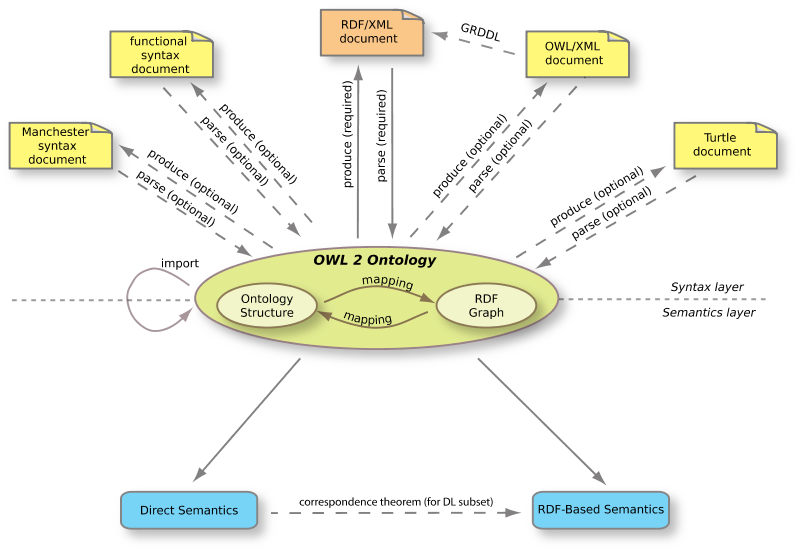
\includegraphics[scale=.45]{OWL2}
%    \caption{The structure of OWL2}
%    \label{fig:OWL2}
%\end{figure}
%
%\section{Conclusion}
%\label {conclusion}
%\input{sections/5_conclusion.tex}
%
%\bibliographystyle{IEEEtran}
%\bibliography{bibliography}

\end{document}
